\documentclass[11pt,letterpaper]{article}
\usepackage{fullpage}
\usepackage[top=2cm, bottom=4.5cm, left=2.5cm, right=2.5cm]{geometry}
\usepackage{amsmath,amsthm,amsfonts,amssymb,amscd}
\usepackage{lastpage}
\usepackage{enumerate}
\usepackage{enumitem}
\usepackage{fancyhdr}
\usepackage{mathrsfs}
\usepackage{mathabx}
\usepackage{siunitx}
\usepackage{graphicx}
\usepackage{listings}
\usepackage{hyperref}
\usepackage{booktabs}
\usepackage{caption,cleveref,colortbl,csquotes,datatool,helvet,mathpazo,multirow,listings,pgfplots,xcolor}

\DeclareSIUnit \erg{erg}
\DeclareSIUnit \au{au}
\DeclareSIUnit \pc{pc}
\DeclareSIUnit \ly{ly}
\DeclareSIUnit \years{years}
\DeclareSIUnit \K{K}

\hypersetup{%
  colorlinks=true,
  linkcolor=blue,
  linkbordercolor={0 0 1}
}

\setlength{\parindent}{0.0in}
\setlength{\parskip}{0.05in}

% edit these
\newcommand\course{CTA200H}
\newcommand\Title{Charting the Growth of Galaxies}
\newcommand\Name{Jeff Shen} 
\newcommand\Id{Dr. Allison Man} 
\newcommand\Date{\today}

\pagestyle{fancyplain}
\headheight 35pt
\lhead{\Name}
\lhead{\Name\\\Id}
\chead{\textbf{\Large \Title}}
\rhead{\course \\ \Date}
\lfoot{}
\cfoot{}
\rfoot{\small\thepage}
\headsep 2em

\begin{document}

% problem 1
\section*{Spectral Fitting}

\begin{figure}[!htbp]
    \centering
    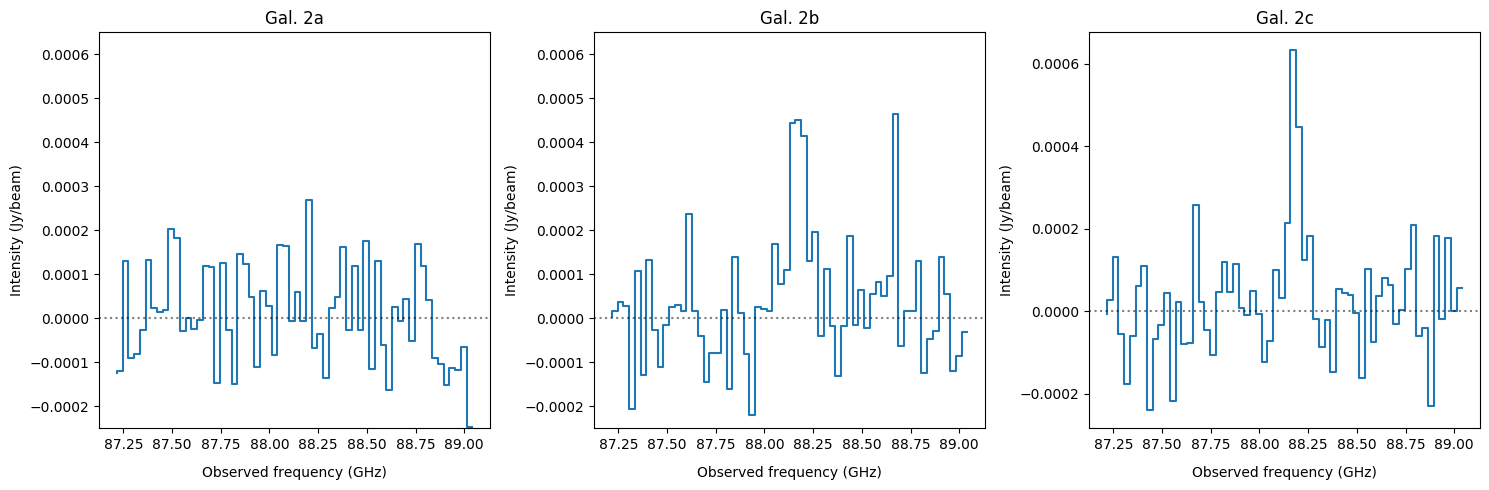
\includegraphics[width=\linewidth]{../figs/initial_spectra.png}
    \caption{Plot of the extracted spectra of the multiple images of Galaxy 2.}
    \label{fig:initial_spectra}
\end{figure}

\begin{figure}[!htbp]
    \centering
    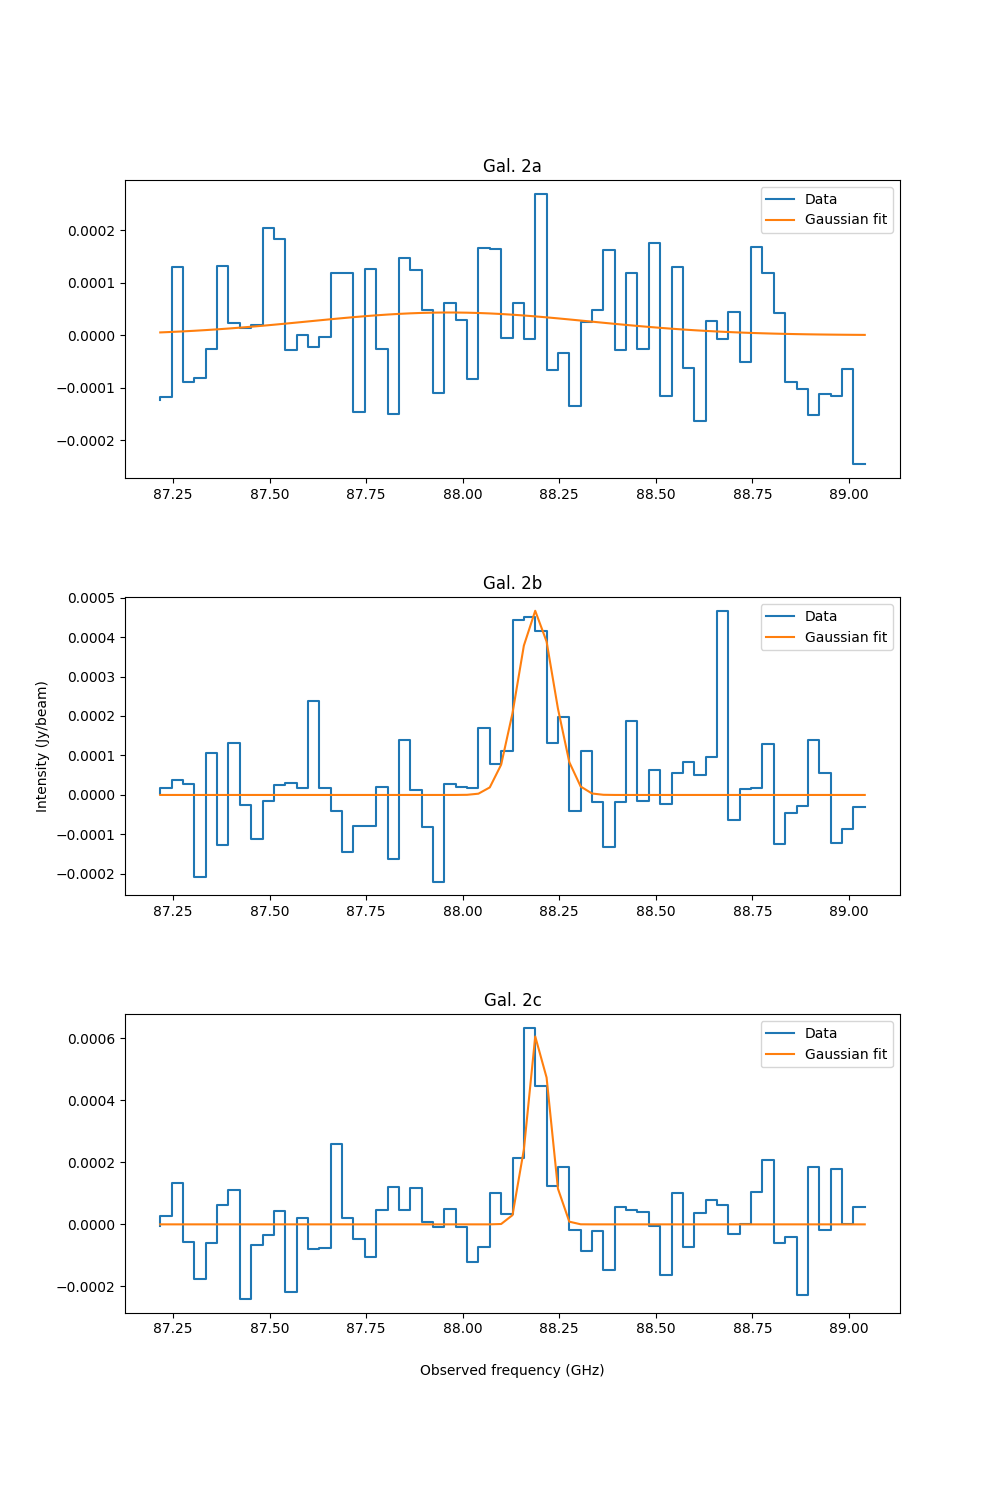
\includegraphics[width=0.8\linewidth]{../figs/gaussian_fit.png}
    \caption{Plot of the spectra with a 1D Gaussian fit.}
    \label{fig:gaussian_fit}
\end{figure}

\begin{figure}[!htbp]
    \centering
    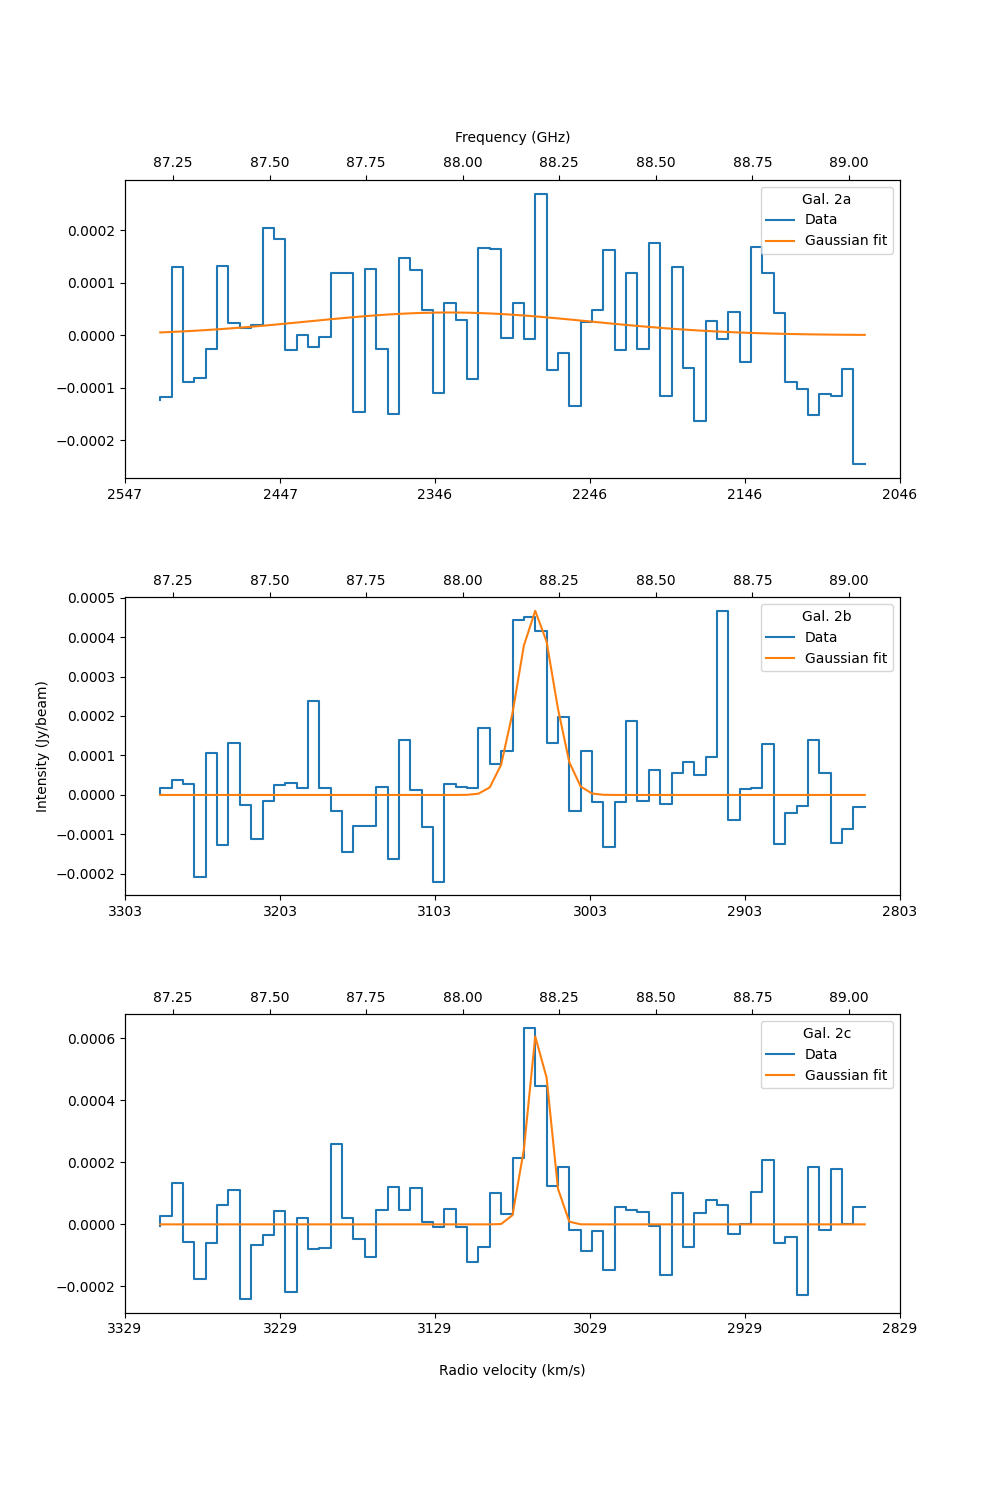
\includegraphics[width=0.8\linewidth]{../figs/redshift_axis_plot.png}
    \caption{Plot of the spectra with a 1D Gaussian fit. Bottom x-axis is in radio velocity (km/s) with reference to the redshift to each image. Top x-axis is in observed frequency (GHz).}
    \label{fig:redshift_axis}
\end{figure}

\begin{table}[!htbp]
\centering
\begin{tabular}{ccccc}
\hline \\[-0.25cm]
Gal & Peak Frequency & Line Width & RMSE & Redshift \\
ID  & GHz            & FWHM       &      & \\[0.1cm]
\hline \\[-0.25cm]
2a & 87.96 & 0.858 & 1.11E-04 & 2.93\\
2b & 88.19 & 0.111 & 1.13E-04 & 2.92\\
2c & 88.20 & 0.064 & 1.06E-04 & 2.92\\
\hline
\end{tabular}
\caption{Table to test captions and labels}
\label{table:1}
\end{table}

% problem 2
\section*{Problem 2: Hot Jupiters and tidal disruption}

\begin{enumerate}[label=(\alph*)]

    \item

    
    \item
    
    
    \item
    
    
    \item

    
\end{enumerate}




\section*{Problem 3:}
\begin{enumerate}[label=(\alph*)]
  
    
\end{enumerate}

\end{document}

